\documentclass[10pt, conference, compsocconf]{IEEEtran}
\usepackage[nocompress]{cite}
\usepackage[font=normalsize,labelfont=sf,textfont=sf]{subfig}
\usepackage{graphicx}
\usepackage{arabtex}
\usepackage[cmex10]{amsmath}

%packages that were not copied from the IEEE template - need to check if it is valid to add them
\usepackage{amssymb}
\usepackage[linesnumbered]{algorithm2e}

%\linespread{1}
%\raggedbottom
%\abovedisplayskip{0.96}

\begin{document}

\title{Real-time Segmentation of On-line Handwritten Arabic Script}

\author{\IEEEauthorblockN{George Kour}
\IEEEauthorblockA{Faculty of Engineering\\
Tel-Aviv University\\
Tel-Aviv Jaffa, Israel\\
Email: georgeko@post.tau.ac.il}
\and
\IEEEauthorblockN{Raid Saabne}
\IEEEauthorblockA{Department of Computer Science\\
Tel Aviv-Yaffo Academic Collage, Israel\\
Triangle R\&D Center, Kafr Qara, Israel\\
Email: saabni@cs.bgu.ac.il}
}

\maketitle

\begin{abstract}
the cursive and unconstrained nature of the Arabic script, in both printed and handwritten forms, anneals the task of segmentation. 
While real-time performance is required in applications involving on-line handwriting recognition, most conventional approaches wait until the entire curve is traced out before starting the analysis, inevitably causing delays in the recognition process. 
This paper proposes a real-time recognition-based segmentation technique of the on-line Arabic script.
It demonstrate the feasibility of carrying out the most time consuming tasks, required for the segmentation process, during the course of writing. 
The system has been designed and tested using the ADAB Database, and promising results were obtained.\\
\end{abstract}

\begin{IEEEkeywords}
Arabic Script Segmentation, Strokes Segmentation, On-line Text Recognition, Word Segmentation, Arabic OCR.
\end{IEEEkeywords}

\section{Introduction}
Handwriting remains the most commonly used mean of communication and recording of information in the daily life, therefore, a growing interest in the handwriting character recognition field has emerged in recent years. 
Handwriting recognition can be categorized into two main fields: off-line and on-line. 
In the off-line case, a digital image containing text is fed to the computer, and the system attempts to convert the spatial representation of the letters into digital symbols \cite{al2011online}. 
In contrast, the process of on-line handwriting recognition is done on a digital representation of the text written on a special digitizer, tablet or smart-phone device, where sensors pick up the pen-tip movements.
 
Research in this field has established two main approaches; the analytic approach, which involves segmentation and classification of each part of the text \cite{abdulla2008off, sari2002off, Dinges2011}, and the holistic approach, which considers the global properties of the written text and recognizes the input word shape as a whole \cite{biadsy2011segmentation, saabni2009hierarchical}. 
While having many advantages, the holistic approach requires the classifier to be trained over the entire dictionary, which is impractical for large dictionaries (containing more than 20,000 words) \cite{elanwar2012unconstrained}.

The cursiveness of the Arabic script, prima facie, requires delaying the launch of the recognition process until the completion of the word scribing. 
However, in this paper, we question the necessity of the requirement by demonstrating the feasibility of approximating the position of the segmentation points (SPs) while the stroke is being written; and by doing so, accelerating the segmentation and, consequently, the recognition process. 
The resulted segmentation and letters classification information can be potentially used to significantly reduce the potential dictionary size and accelerate a later holistic recognition process.

In Section \ref{sec:related_work}, we mention related studies done in the field of on-line Arabic recognition. 
The proposed approach is described in detail in Section \ref{sec:approach}. Experimental results and analysis is given in Section \ref{sec:results}. 

\section{Related Work}
\label{sec:related_work}

The research in on-line handwriting recognition started in the 1960's and has been receiving a great interest from the 1980's \cite{tagougui2013online}. 
One of the earliest studies on On-line Arabic script recognition was carried out by El-Wakil and Shoukry in 1989 \cite{el1989line}.

Randa et al. \cite{elanwar2012unconstrained} proposed a two stage on-line Arabic handwritten text segmentation system based on Hidden Markov Model (HMM). 
In the first stage, SPs were nominated, and then, in a second stage, the nominated points were validated using a rules-based engine. 
The system was tested using a self-collected database named OHASD.

Digness et al. \cite{Dinges2011} used a segmentation-based recognition approach based on dividing the word into smaller pieces, which were afterwards segmented into candidate letters, and then classified into letter classes, using statistical and structural features. 
A $k$ nearest neighbor ($k$-NN) classifier was used to obtain the final recognition.

A segmentation-based recognition method that operates on the stroke level for on-line Arabic handwritten words recognition was proposed by Daifallah et al. \cite{daifallah2009recognition}. 
SPs were nominated and then selected by locating semi-horizontal lines moving from right to left. 
A portion of the SPs is filtered out by applying a certain set of rules. 
Then, HMM is used to classify the sub-strokes to letters using the Hu feature. 
The letters candidates and their scoring were used to determine the best set of SPs.

A recent survey, done by Tagougui et al. \cite{tagougui2013online}, reviews the status of research in on-line Arabic handwriting recognition field. 

\section{Our Approach}
\label{sec:approach}

\textbf{Complexity measure:} this value indicates the curvature degree of a given 2-D trajectory. 
As we shall see, this measure will be found useful in several stages through the segmentation flow.
In order to avoid this measure from being affected by vibrations and data imperfection, the trajectory undergone a simplification process using the Douglas-Peucker algorithm \cite{douglas1973algorithms}.
The complexity measure is calculated by summing the parameters $\alpha_{k}$ computed for each inner point $p_k$ in the simplified version, $T=\{p_i\}_{i=1}^{n}$, of the original trajectory obtained by the digitizer.
Namely, $CM(T)=\sum_{k=2}^{n-1}{\alpha_k}$, where $\alpha_{k}=C(1-\frac{\phi_k}{\pi})$, $\phi_k=\angle(\overline{p_{k-1}p_{k}},\overline{p_{k}p_{k+1}})$, and $C$ is a constant which was experimentally set to 6.\\

The proposed approach goes through three stages. 
In the first stage, \emph{points of interest} (POIs), are continuously nominated while the stroke is being scribed.
The sub-strokes imposed by these POIs are scored by an Arabic letter classifier. 
In the second stage, once the entire stroke is available, a rules-based process is used to refine the set of POIs and re-score the sub-strokes. 
Eventually, the system heuristically determines the final set of SPs based on the sub-strokes scoring. See Figure \ref{fig:system_flow}. 

\begin{figure}
\centering
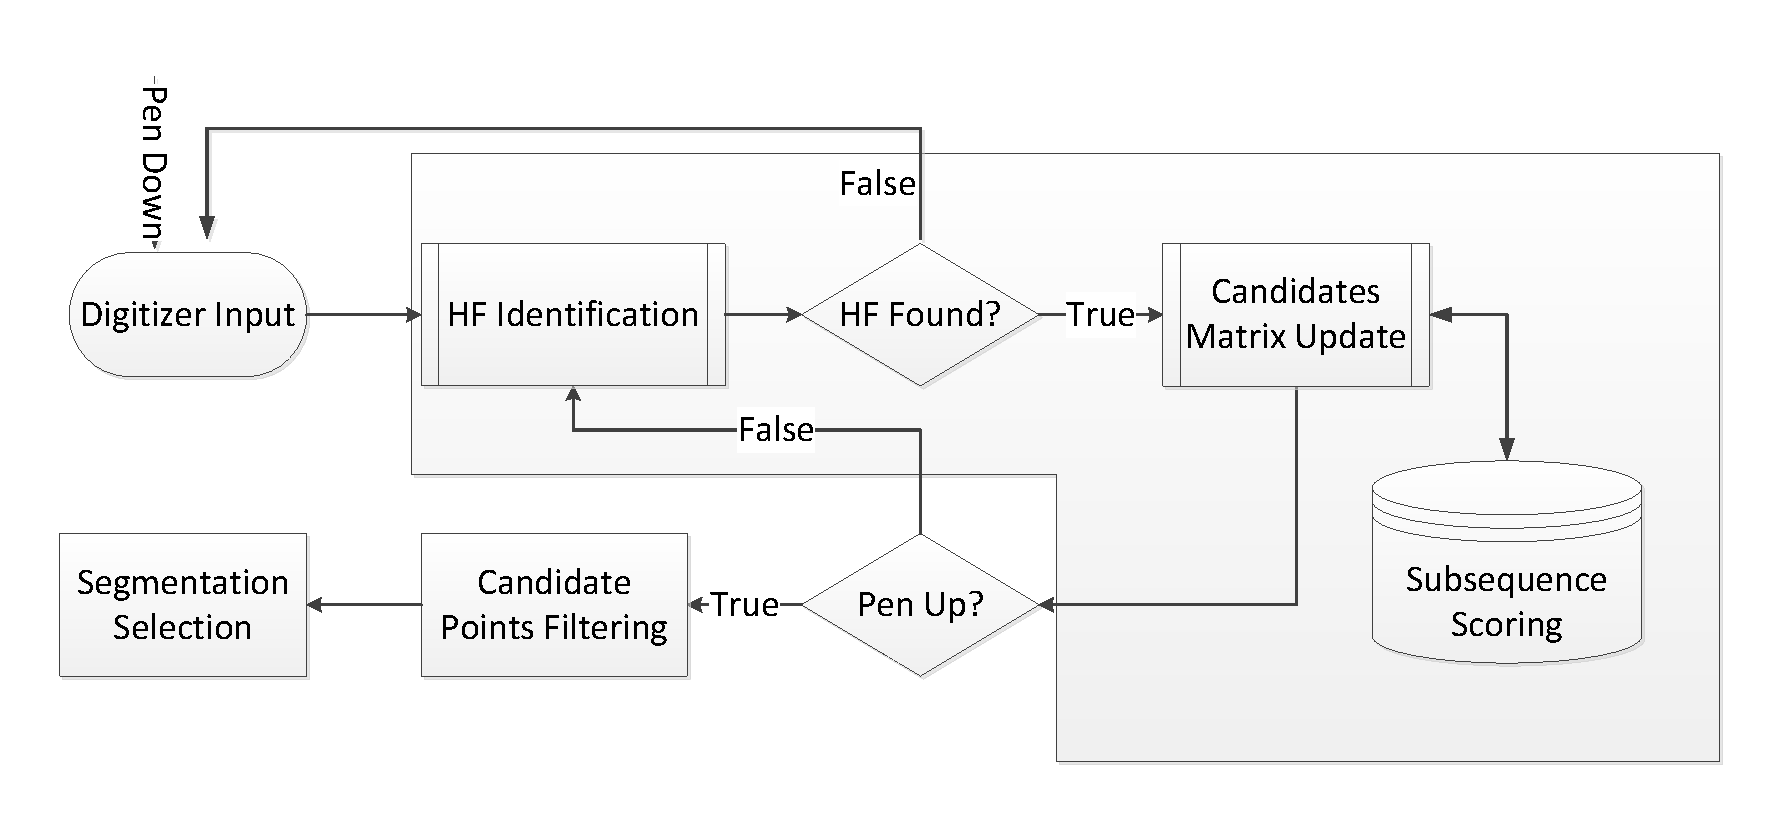
\includegraphics[width=1\columnwidth]{./figures/system_flow}
\caption{High level visualization of the system flow.}
\label{fig:system_flow}
\end{figure}

\subsection{First Stage: POIs Nomination and Sub-strokes Scoring}

\textbf{Horizontal fragment identification:} in this stage, the system attempts to identify \emph{horizontal fragments} (HFs) that join pairs of connected letters in the Arabic script. 
These handlers are usually horizontal, directed right to left, and located near the baseline. 
Using a smoothed version of the trajectory, obtained by using splines interpolation method, helps the process to ignore undesired small horizontal regions that are frequently caused by the digitizer.  
A point $p_{i}$ is defined as a "horizontal point" if the slope of the line $\overline{p_{i-1}p_{i}}$ is less than a preset value $\delta$, which was empirically tuned to $0.6$. 
The same exact value for this parameter was found independently in \cite{daifallah2009recognition}.

%\begin{figure}
%\centering
%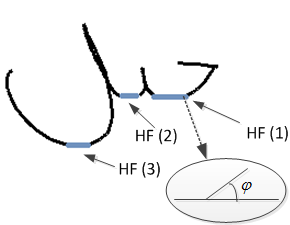
\includegraphics[width=0.4\columnwidth]{./figures/horizontal_fragments}
%\caption{Horizontal Fragments [HF] of the word \RL{jbl} (JABAL).}
%\label{fig:horizontal_fragments}
%\end{figure}

HFs are continuously identified using the following process.
The first detected horizontal point is set as an "HF starting point". 
All subsequent horizontal points are ignored until a non-horizontal point is detected, indicating the end of an HF sequence. 
This point is identified as an "HF ending point" and the medial point of an HF is marked as POI. 
POIs are potential SPs, thus, this process yields an over-segmentation of the stroke. 
While false positive SPs can be easily removed, missed real SPs cannot be easily recovered. 
Therefore, in order to minimize the miss-rate, this process is delicate and allows false HFs to be detected.

In a post processing step, fractions of the same horizontal segment, which were identified as multiple HFs, are rejoined to a single HF. 
The merging is done by evaluating the complexity measurement between the two consequent HFs.

\textbf{Sub-strokes scoring:}
Let $S=\{p_{i}\}_{i=1}^{n}$ be a sequence representing a handwritten stroke in which $L$ POIs were detected. 
Let $KP=\{KP_{i}\}_{i=0}^{L+1}$ (Key points) be the ordered set of POIs, in addition to the first and the last points of the stroke positioned as the first and the last items in the set.
Formally, we define: 
\begin{equation}
KP_{i} =\begin{cases}    1		, & \mbox{if } i=0 \\
							   POI_{i}	, & \mbox{if } 1\leq i \leq L \\
							   n    , & \mbox{if } i=L+1 
			\end{cases}				
\end{equation}
A sub-stroke $S_{i}^{j}$ is a sub-sequence of the stroke $S$ that starts at $KP_{i}$ and ends at $KP_{j}$, formally:
\begin{equation}
S_{i}^{j}=\{p_{k}\}_{k=KP_{i}}^{KP_{j}}; i<j
\label{eq:substroke_definition}
\end{equation}

We generate an upper triangular scoring matrix $D\in\mathbb{R}^{(L+1)\times (L+1)}$ where each cell $D_{i,j}$ represents the sub-stroke $S_i^j$. It contains the information returned by the scoring system for the sub-strokes $S_i^j$. 
The matrix $D$ is generated dynamically; adding a row and a column for each new detected POI. 
Imposing a locality constraint which narrows the band of the $D$ matrix above the main diagonal improved the efficiency of the process and the segmentation accuracy. 
Given a band width $B$ we fix $D_{i,j}=\infty$ if  $j \leq i$ or $j-i>B$.
We argue that sub-strokes representing a letter will achieve, in most cases, better scoring, i.e., lower $D_{i,j}$ value than other sub-strokes.

\begin{figure}
\centering
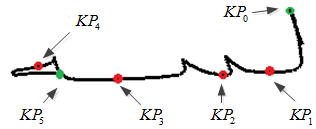
\includegraphics[width=0.6\columnwidth]{./figures/candidate_points}
\caption{KPs of the word \RL{lbyh} (Lbyh). POIs are colored in red. The first and last key points (KPs) are colored in green. }
\label{fig:candidate_points}
\end{figure}

The classifier contains four databases, one for each letter position (Ini, Mid, Fin and Iso). 
It receives a sequence of points representing the sub-stroke and a letter position, and outputs a list of sample candidates and their scoring which indicates the similarity measure between the sequence and the candidate.
The real-time nature of the segmentation technique strictly requires the classifier to be extremely fast.
The compliance with the high performance demand was made possible by using a state-of-the-art method for fast computation of the approximate $k$-NN, based on the technique proposed in \cite{saabni2013efficient}.
The relative location of the sub-stroke in the stroke, was used to avoid accessing all the four databases. 
As can be seen in Table \ref{table:subsequences_types}, we differentiate between four types of subsequences. 
For each type, we indicate the set of databases that need to be examined, i.e., the possible letter positions the sub-stroke may represent. 

\begin{table}
\centering
\renewcommand{\arraystretch}{1.5}
\caption{A mapping between the subsequence types and the possible letter positions. $S$ denotes a stroke containing $L$ POIs. $S_i^j$ is defined in Equation \ref{eq:substroke_definition}, $m>0$ and $k<L+1$. }
\begin{tabular}{| c |c | c |}
\hline
  Name     & Subsequence    & Letter Position       \\
\hline
  $\alpha$ & $S_0^{k}$         & $Ini$ or $Mid$  \\
\hline
  $\beta$  & $S_{m}^{k}$     & $Mid$              \\
\hline
  $\chi$    & $S_{m}^{L+1}$ & $Mid$ or $Fin$   \\
\hline
  $\delta$ & $S_0^{L+1}$     & All                   \\
\hline
\end{tabular}
\label{table:subsequences_types}
\end{table}

The relation between the cells in the matrix $D$ and the sub-stroke type is given in matrix $D_p$  (Equation \ref{eq:positions_matrix}). 
The type of the sub-stroke can be determined while the stroke is being scribed.
The last column and row are added on the "pen up" event.
\begin{equation}
D_{p}=
\left( 
\begin{array}{ccccccc}
\infty 	& \alpha & \alpha & \alpha  & \cdots & \alpha & \delta \\
\infty  & \infty  & \beta   & \beta   & \cdots  & \beta  & \chi    \\
\infty  & \infty  & \infty   & \beta   & \cdots  & \beta  & \chi    \\
\vdots & \vdots & \vdots  & \vdots & \ddots  & \vdots & \vdots \\
\infty  & \infty  & \infty   & \infty   & \cdots  & \beta  & \chi    \\
\infty  & \infty  & \infty   & \infty   & \cdots  & \infty  & \chi    \\
\infty  & \infty  & \infty   & \infty   & \cdots  & \infty  & \infty \end{array} \right)
\label{eq:positions_matrix}
\end{equation}

For a given input (sequence and position), the recognition system returns the $K$ nearest neighbors with different labeling, where the labeling is defined as the tuple (letter, position). In our implementation, we set $K=3$.

\begin{figure}
\centering
\renewcommand{\arraystretch}{1.2}
\begin{tabular}{| c |c | c | c| c | c | c |}
\hline
     & $0$ & $1$ & $2$ & $3$ & $4$ & $5$\\
\hline
$0$
   & N/A
   & \subfloat{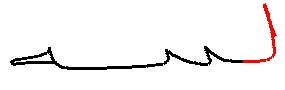
\includegraphics[width=0.8cm]{./figures/substrokes/L}}
   & \subfloat{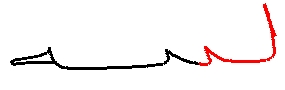
\includegraphics[width=0.8cm]{./figures/substrokes/LB1}}
   & \subfloat{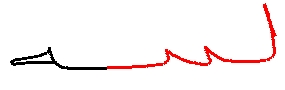
\includegraphics[width=0.8cm]{./figures/substrokes/LB1B2}}
   & N/A & N/A \\
\hline
$1$
   & N/A & N/A
   & \subfloat{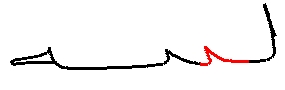
\includegraphics[width=0.8cm]{./figures/substrokes/B1}}
   & \subfloat{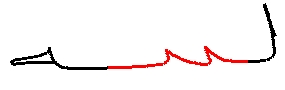
\includegraphics[width=0.8cm]{./figures/substrokes/B1B2}}
   & \subfloat{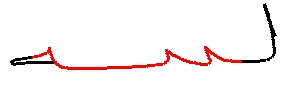
\includegraphics[width=0.8cm]{./figures/substrokes/B1B2H1}}
   & N/A \\
\hline
$2$
   & N/A  & N/A & N/A
   & \subfloat{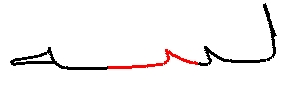
\includegraphics[width=0.8cm]{./figures/substrokes/B2}}
   & \subfloat{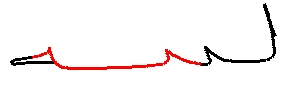
\includegraphics[width=0.8cm]{./figures/substrokes/B2H1}}
   & \subfloat{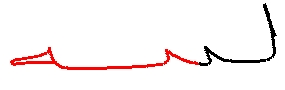
\includegraphics[width=0.8cm]{./figures/substrokes/B2H}} \\
\hline
$3$
   & N/A & N/A & N/A & N/A
   & \subfloat{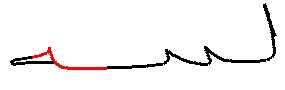
\includegraphics[width=0.8cm]{./figures/substrokes/H1}}
   & \subfloat{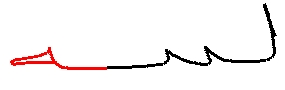
\includegraphics[width=0.8cm]{./figures/substrokes/H}} \\
\hline
$4$
   & N/A & N/A & N/A & N/A & N/A
   & \subfloat{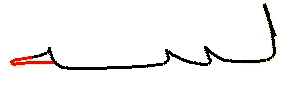
\includegraphics[width=0.8cm]{./figures/substrokes/H2}}\\
\hline
$5$
   & N/A & N/A & N/A & N/A & N/A & N/A \\
\hline
\end{tabular}
\caption{A tabular representation of the $D$ matrix that corresponds the KPs showed in Figure \ref{fig:candidate_points}. Each cell visually demonstrates the corresponding sub-stroke colored in red.}
\label{table:substrokes_demo} 
\end{figure}

\subsection{Second Stage: Candidate points filtering and scoring correction}
In this stage we re-score subsequences and eliminate redundant POIs based on the following rules:

\begin{enumerate}
	\item Inner SPs should lie close to the baseline. 
	\item SPs do not reside in loops.
	\item The sub-stroke length should be proportional to the length of the containing stroke.
\end{enumerate}

\textbf{Baseline detection:} The system determines the baseline by calculating the vertical density histogram of the re-sampled and normalized sub-stroke. 
The height of the stroke (y-axis) is partitioned into ten equi-length intervals. 
A POI is filtered out if it does not satisfy the following condition:
\begin{equation}
|POI_y-I_{max}| \leq 2*max{({|I|},0.15)}
\end{equation}
where $POI_y$ represents the $y$-coordinate of the POI, $|I|$ is the length of an interval, and $I_{max}$ denotes the center of the most inhabited interval. 
In order to reliably determine the baseline, the algorithm is activated only after the fourth POI is detected. 
This process has proven to be very effective in eliminating challenging false POIs that reside in valleys of frequently used final Arabic letters, such as \RL{-q}, \RL{-s} and \RL{-n}. 
An example of such a POI can be seen in the letter \RL{-n} in Figure. 
The baseline is needed only to verify that the POIs are in a reasonable distance from it, therefore, imprecise valuation of the position or the direction of the baseline is tolerable.\\

The third rule is used to penalize unreasonably low scoring given to small sub-strokes, which are unlikely to represent a letter. 
This is done by calculating the ratio of the sub-stroke length proportional to the entire stroke length.
For instance, it is common to add a small, hook-like, extension to the suffix of the letter \RL{d} that may look very similar to the letter \RL{-a} during the stroke scribing; and thus under-scored by the recognition system, and eventually, result in over-segmenting the letter \RL{d}. 
%In some cases, POIs are incorrectly nominated on non-horizontal areas. This is caused due to noises in the data and the fact that the nomination is done while the word is being scribed. 
Our filtering algorithm should be corrected, in a future work, to handle this case.

\subsection{Third Stage: Segmentation Selection}
The goal of this phase is to select the \emph{final segmentation points} (FSP) among the POIs. 
It is performed by finding the \emph{segmentation path} in $D$ with the best scoring possible. 
A segmentation path $\pi$ is an ordered subset of the KPs that must contain $KP_{0}$ and $KP_{L+1}$ as the first and the last points in the path.
$\Pi$ denotes the scoring of the segmentation path $\pi$. 
It is defined as the summation of the sub-sequences scoring in the segmentation path divided by the path length; this is done in order to prevent giving superiority to under-segmentations.

One can model the scoring matrix $D$ as a directed, edge-weighted graph $G=(V,E)$, for which a path from vertex $KP_0$ to vertex $KP_{L+1}$ defines a possible segmentation. 
It can be experimentally validated that finding the shortest path in $G$ (from $KP_0$ to $KP_{L+1}$) does not necessarily obtain the optimal segmentation, and in some cases, produces under-segmentation of the stroke. 
It is because the shortest path is a global property, which may prefer a highly weighted shortcut path over a path that consists of several low weighted fragments; in cases where the accumulative weight of the fragmented path is larger than the shortcut path.
However, greedily selecting the outgoing edge with the minimal weight will mostly return a better segmentation.

Several \emph{segmentation selection algorithms} (SSAs) for finding the best segmentation path are proposed in this work.
Here we describe two algorithms that were given the names \emph{Forward Segmentation Selection} (FSS) and \emph{Backward Segmentation Selection} (BSS) which operate quite similarly. 
A pseudo-code of FSS algorithm can be seen in Algorithm \ref{alg:fss}. 
FSS starts with the first point, $KP_0$, advancing toward the end of the stroke. 
In Each step, it tries to find the next best KP by selecting the adjacent subsequence $S_i^j$ with the best scoring (as can be seen in line 5). 
BSS operates similarly but starts from the last point and advances toward the beginning of the stroke. 
The main drawback of these two algorithms is that FSS tends to under-segment the suffix of the stroke and BSS tends to under-segment the stroke's prefix.

In an attempt to overcome the aforementioned drawbacks, a third SSA is proposed, which given the name \emph{Backward-Forward Segmentation Selection} (BFSS). 
As can be seen in Algorithm \ref{alg:bfss}, it combines both FSS and BSS.
BFSS operates from the sides of the stroke toward the center. In every iteration, it selects two candidate points to include to the segmentation path.

The last algorithm was given the name \emph{Greedy Segmentation Selection} (GSS) and is described in Algorithm \ref{alg:gss}, operates differently.
In every iteration, the cell with the lowest (best) scoring is selected. 
Once a cell $D_{i,j}$ is selected, since it represents the sub-stroke $S_{i}^{j}$, both $KP_{i}$ and $KP_{j}$ are added to the FSP, and every cell corresponding to a subpart of the sub-stroke $S_{i}^{j}$ is removed by setting its corresponding scoring value in the matrix $D$ to $\infty$; in order to avoid those sub-strokes to be selected in a later iteration. In Algorithm \ref{alg:gss}, the notation $[\infty]^{(L+1)\times (L+1)}$ indicates a matrix that all it's cells are set to $\infty$.

Performance evaluation of the mentioned SSA is provided in Section \ref{subsec:ssa_performance}.

\begin{algorithm}
$\pi = \{0\} $\;
$i=0$\;
$sum=0$\;
\While{$i<L+1$}
{
	$j = \mathop {\arg \min }\limits_k \left( {D\left( {i,k} \right)} \right)$\;
	$\pi = \pi \cup \left\{ j \right\}$\;
	$sum = sum + D\left( {i,j} \right)$\;
	$i=j$\;
}
\caption{Forward Segmentation Selection.}
\label{alg:fss}
\end{algorithm}

\begin{algorithm}
$\pi = \{0,L+1\}$\;
$kp_{a}=0$\;
$kp_{b}=L+1$\;
\While{$kp_{a}<kp_{b}$}
{
	$kp_{a,next} = \mathop {\arg \min}\limits_k (D(kp_a,k))$\;
	$\pi = \pi \cup \{kp_{a,next}\}$\;
	$kp_{a}=kp_{a,next}$\;
	
	$kp_{b,next} = \mathop {\arg \min}\limits_k (D(k,kp_{b,next}))$\;
	$\pi = \pi \cup \{kp_{b,next}\}$\;	
	$kp_{b}=kp_{b,next}$\;
}
\caption{Backward-Forward Segmentation Selection.}
\label{alg:bfss}
\end{algorithm}

\begin{algorithm}
$\pi = \{0,L+1\}$\;
\While{$D \neq [\infty]^{(L+1)\times (L+1)}$}
{
	${s,e} = \mathop {\arg \min}(D)$\;
	$\pi = \pi \cup \{s,e\}$\;
	$sum = sum + D(s,e)$\;
	$UpdateMatrix(D,s,e)$\;
}
\caption{Greedy Segmentation Selection.}
\label{alg:gss}
\end{algorithm}

\section{The ADAB Database}
\label{sec:database}
The ADAB database, described in \cite{el2009icdar}, is a de-facto standard in the field of on-line Arabic handwriting recognition. 
It is freely available and consists of more than 20k Arabic handwritten words (937 Tunisian town/village names) scribed by more than 170 different writers. 

Unfortunately, the ADAB only provides data on the strokes for a given city name. 
No segmentation into letters or \emph{word parts} (WPs) is provided by the database, thus, extra work was needed to add this information in order to use its letter samples and as a ground truth for the segmentation system.
To provide this information, we employed the skills of a human expert to segment the strokes into letters, and to determine the words and the WP boundaries for each sample. 
This additional information was saved in an XML file. 
Delayed strokes were not included in the processed information since it is not considered by the segmentation process.
We have manually segmented more than 7k samples which consisted about 20k strokes. 

%\begin{figure}
%\centering
%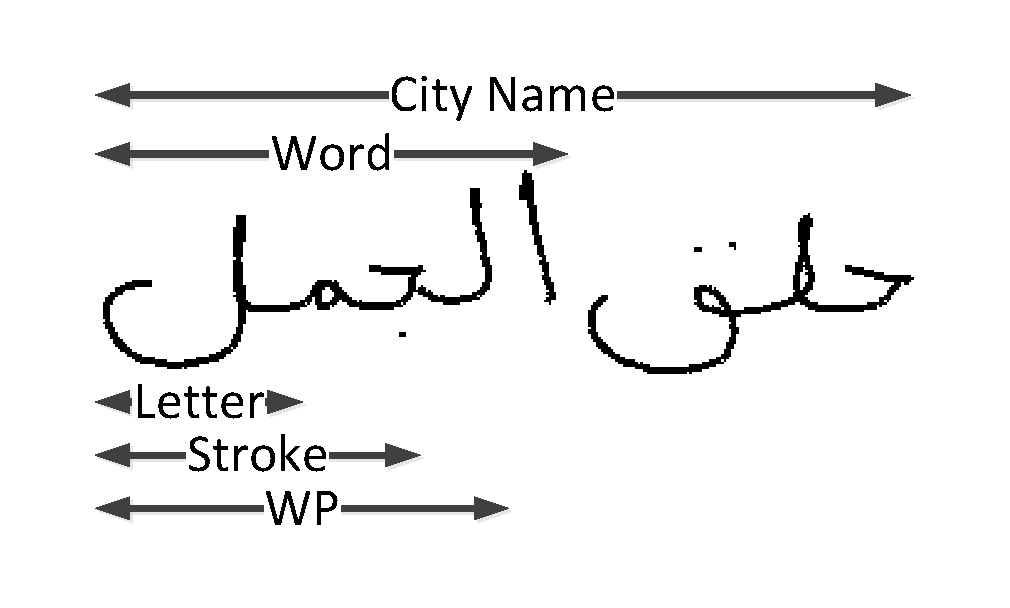
\includegraphics[width=0.7\columnwidth]{./figures/sample_parts}
%\caption{The different parts of a sample in the ADAB database.}
%\label{fig:sample_parts}
%\end{figure}

\section{Validation}
\label{sec:validation}
Related researches usually use a human expert to validate the accuracy of the SPs. However, in this work, we applied an automatic validation process using the ground truth information provided by the database. We discriminate between three types of final SPs. A final SP is classified as true positive if the complexity measure between the identified point and a true SP is less than a preset threshold; otherwise, it is classified as false positive. A false negative (miss), is the case when the system failed to identify a true SP.
The validation process was tested on several sets and found to be highly reliable.

%\begin{figure}
%\centering
%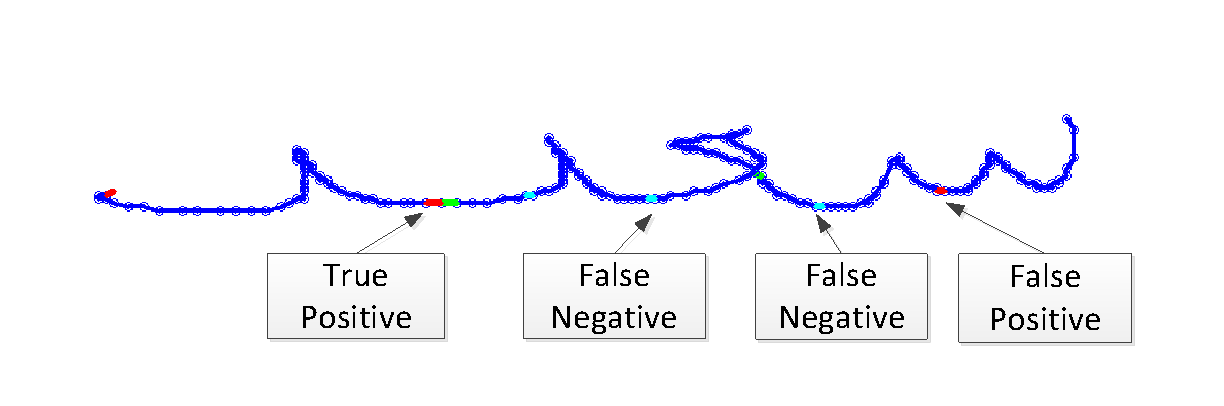
\includegraphics[width=0.9\columnwidth]{./figures/sp_types}
%\caption{SPs types.}
%\label{fig:sp_types}
%\end{figure}

\section{Experimental Results}
\label{sec:results}
The system was implemented using Matlab environment. 
Comparing the performance of the proposed approach to results obtained by related researches could be difficult due to the different experimental settings, databases and methodology; not to mention the different measures used to present the results. 
The usage of the ADAB database, instead of a self-collected database, standardize and reinforces our results. 
In Table \ref{table:general_stats_results} we provide basic statistics of our sample set and summarizes the system's performance.

\begin{table}[h]
\caption{General statistics and results}
\renewcommand{\arraystretch}{1.2}
\begin{tabular}{ | c | c | }
  \hline
  Number of test samples (city names) & 319 \\
  \hline
  Number of WPs & 1148 \\
  \hline
  Number of Strokes & 1237 \\
  \hline
  Strokes segmentation rate (SR) &  83\% \\ 
  \hline
  Strokes recognition rate (RR) &  78\% \\ 
 \hline
  Total number of true SPs & 1081 \\
  \hline
  Valid SPs (True Positive) & 85.3\% \\
    \hline
  Missing SPs (False Negative) & 14.7\% \\
  \hline
  Invalid SPs (False Positive) & 119 (11\%) \\
  \hline                                    
  SPs Precision & 88.6\% \\ 
 \hline
  SPs Recall &  85.3\% \\ 
  \hline
\end{tabular}
\centering
\label{table:general_stats_results} 
\end{table}

It is important to note that the absolute majority of the false negative (missed) SPs were identified as POIs in the first stage.
However, most of them, were not selected by the SSA.
A small number were filtered out in the filtering phase. 

%\begin{table}[h]
%\caption{Results}
%\renewcommand{\arraystretch}{1.2}
%\begin{tabular}{ | c | c | }
%  \hline
%  Strokes segmentation rate (SR) &  83\% \\ 
%  \hline
%  Strokes recognition rate (RR) &  78\% \\ 
% \hline
%  Total number of true SPs & 1081 \\
%  \hline
%  Valid SPs (True Positive) & 85.3\% \\
%    \hline
%  Missing SPs (False Negative) & 14.7\% \\
%  \hline
%  Invalid SPs (False Positive) & 119 (11\%) \\
%  \hline                                    
%  SPs Precision & 88.6\% \\ 
% \hline
%  SPs Recall &  85.3\% \\ 
% \hline
%\end{tabular}
%\centering
%\label{table:results} 
%\end{table}

\subsection{Analysis}
In this section we discuss common cases of incorrect segmentation.
\subsubsection{Over-segmentation}
\begin{itemize}
\item Several Arabic letters contain a horizontal region in their initial form which does not accommodate a SP. We overcame this problem by adding the following rule: a POI is nominated only if the sub-stroke that spans from the beginning of the stroke to the POI has a high complexity measure.
\item Over-segmentation can also be caused by typing a letter in unusual form where it is spanned over several strokes. 
It happens mostly in the letter \RL{-m-}, \RL{-m} and in rare cases in the letter \RL{-.h-}. This issue will be addressed in a future work.
\end{itemize}

\subsubsection{Under-segmentation}
\begin{itemize}
\item Letter pairs that are not separated by HFs cause the system to miss POIs. This was partially solved by extending the notion of a letter to include such pairs. For example the pair \RL{lm} and \RL{l.h}.
\item In some cases, HFs were identified correctly but the corresponding POI were not selected in the third stage. 
\end{itemize}

In addition, differentiating between the main body of the letter \RL{-s-} and the main body of two consecutive \RL{-b-} letters is possible only when considering additional strokes, thus both cases were considered to be correct.

\begin{figure}
\centering
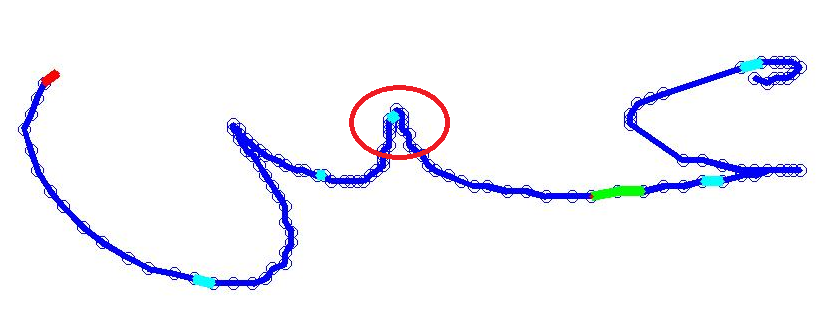
\includegraphics[width=0.5\columnwidth]{./figures/candidate_in_no_horizontal}
\caption{The main body of Arabic word \RL{`yn} (AIN). POIs are colored in cyan. The green areas indicate merge between two subsequent HFs. Three types of false POIs can be seen: 1. A POI at the beginning of a stroke. 2. A POI that is caused by a bad HF. 3. A POI that resides in a letter's valley. }
\label{fig:candidate_in_no_horizontal}
\end{figure}

\subsection{Segmentation Selection Algorithms Performance}
\label{subsec:ssa_performance}
As can be seen in Table \ref{table:ss_algorithms_results}, the SSA crucially effect on the system's performance. 
We tried different combinations of two SSAs in which the FSP is done by running both SSAs independently and selecting the segmentation path with the smallest scoring. 
In Table \ref{table:ss_algorithms_results}, a combination of two algorithms is denoted by $\oplus$.

\begin{table}
\caption{SSAs Performance}
\renewcommand{\arraystretch}{1.2}
\begin{tabular}{ | c | c | c | c | c |}
\hline
SSA & WP SR & WP RR & SP Precision & SP Recall\\
\hline                 
  FSS & 76\% & 70\% & 85\% & 78\% \\ 
  \hline
  BSS & 79\% &  73\% & 84\%& 81\% \\
  \hline
  BFSS & 78\% & 72\% & 84\% & 80\%\\ 
  \hline
  GSS & 80\% & 74\% & 81\% & \bf{94}\% \\  
  \hline
  FSS$\oplus$BSS & \bf{82}\% & \bf{76}\% & \bf{89}\% & 82\%\\  
  \hline
  GSS$\oplus$BFSS & 81\% & 75\% & 83\% & 90\% \\
  \hline
\end{tabular}
\centering
\label{table:ss_algorithms_results} 
\end{table}

\subsection{Sample set size and distribution}
The letters is our training set are extracted from a database with a limited words diversity, thus, the distribution of the samples between the different classes is imbalanced. 
On one hand, it can be regarded as an advantage; since, the training set distribution reflects the a-priory probability of a letter appearance in the test set. 
On the other hand, a highly imbalanced training set is known to negatively affect many classification algorithms.
In the following experiment, we measure the effect of a large and imbalanced training set on the WP segmentation and recognition rates. 
It is done by gradually increasing the maximal allowed number of samples per class (letter and position).
 
The graph in Figure \ref{fig:num_letter_impact} shows convergence of the system's performance when the maximal number of samples is larger than 200 per class. 
Nevertheless, a miniature degradation can be seen, which is caused, probably, due to the increasing imbalance in the distribution of the training set.
In addition, it is evident that the recognition rate (RR) is more sensitive to small training set than the segmentation rate (SR).

\begin{figure}
\centering
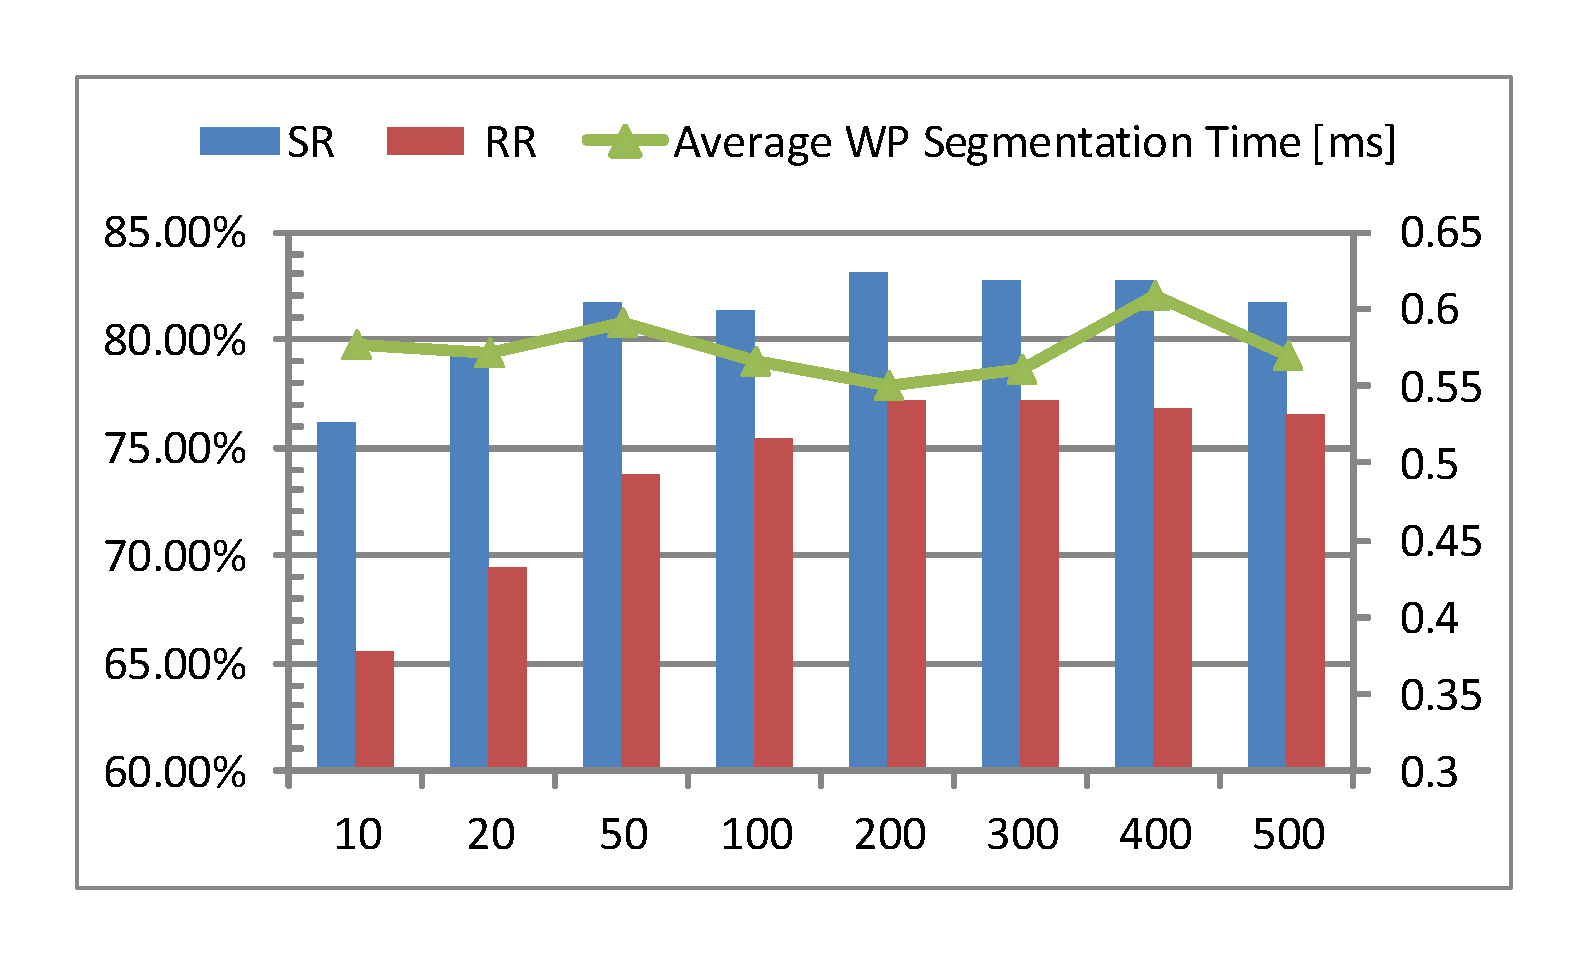
\includegraphics[width=1\columnwidth]{./figures/num_letter_impact}
\caption{The impact of increasing the maximal number of samples per class on the segmentation and recognition rates.}
\label{fig:num_letter_impact}
\end{figure}

\section{Summary and Future Work}
In this paper, we proposed a novel real-time approach for segmenting open-dictionary, Arabic handwritten script.
The segmentation is performed in the strokes level. 
Morphological features are employed to nominate potential SPs. 
The sub-strokes induced by the SPs are classified using a $k$-NN letters classifier, and the classification information is saved in a scoring matrix.
The final segmentation points are then selected by finding the best-scored segmentation path in the scoring matrix. 
This is done using several proposed algorithms. 
The system has demonstrated promising results.

In future work, we will expand the process by adding a later holistic WP recognizer that exploits the proposed segmentation and the scoring information to inspect a limited number of potential WPs.

\section*{Acknowledgment}
The authors would like to thank Professor Dana Ron, from the Tel-Aviv University, for her invaluable help in this research and her insightful comments on this paper. 

\bibliographystyle{IEEEtran}
\bibliography{IEEEabrv,bibliography}

\end{document}


